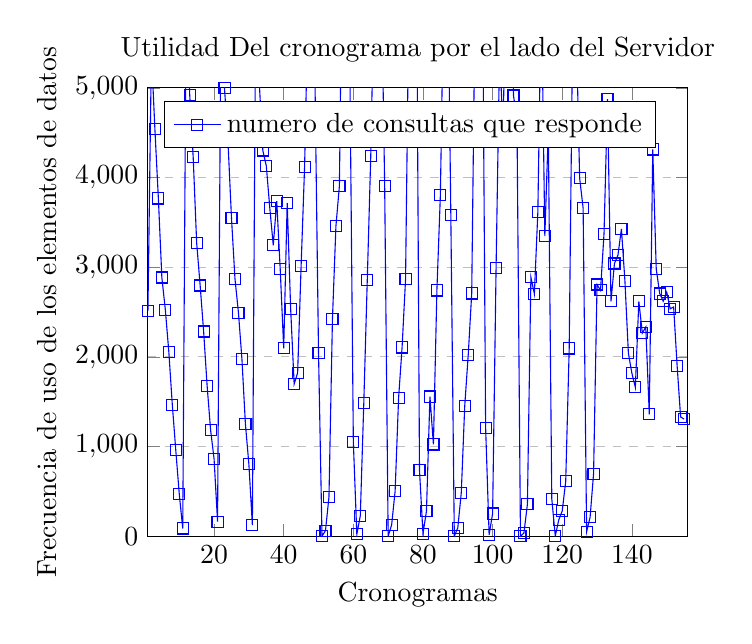
\begin{tikzpicture}
\begin{axis}[
    title={Utilidad Del cronograma por el lado del Servidor},
    xlabel={Cronogramas},
    ylabel={Frecuencia de uso de los elementos de datos},
    xmin=1, xmax=156,
    ymin=0, ymax=5000,
    xtick={},
    ytick={},
    legend pos=north west,
    ymajorgrids=true,
    grid style=dashed,
]

\addplot[
    color=blue,
    mark=square,
    ]
    coordinates {
%UTILIDAD TOTAL
(1,2512)
(2,5401)
(3,4540)
(4,3767)
(5,2885)
(6,2525)
(7,2057)
(8,1467)
(9,959)
(10,470)
(11,86)
(12,6082)
(13,4924)
(14,4226)
(15,3270)
(16,2796)
(17,2283)
(18,1678)
(19,1184)
(20,861)
(21,162)
(22,5999)
(23,4994)
(24,4392)
(25,3550)
(26,2871)
(27,2493)
(28,1975)
(29,1251)
(30,801)
(31,123)
(32,6266)
(33,5048)
(34,4302)
(35,4130)
(36,3662)
(37,3244)
(38,3736)
(39,2976)
(40,2095)
(41,3717)
(42,2531)
(43,1697)
(44,1821)
(45,3015)
(46,4120)
(47,5963)
(48,6423)
(49,5030)
(50,2045)
(51,0)
(52,62)
(53,438)
(54,2425)
(55,3459)
(56,3907)
(57,7339)
(58,5847)
(59,5234)
(60,1049)
(61,21)
(62,228)
(63,1481)
(64,2854)
(65,4236)
(66,6177)
(67,5847)
(68,6366)
(69,3905)
(70,0)
(71,126)
(72,502)
(73,1542)
(74,2105)
(75,2867)
(76,6159)
(77,7137)
(78,7610)
(79,734)
(80,28)
(81,278)
(82,1557)
(83,1023)
(84,2741)
(85,3805)
(86,6245)
(87,6809)
(88,3582)
(89,0)
(90,93)
(91,482)
(92,1455)
(93,2022)
(94,2707)
(95,6084)
(96,6980)
(97,6890)
(98,1206)
(99,16)
(100,252)
(101,2995)
(102,5396)
(103,4537)
(104,6541)
(105,6904)
(106,4914)
(107,4646)
(108,0)
(109,35)
(110,358)
(111,2888)
(112,2703)
(113,3620)
(114,6143)
(115,3347)
(116,4526)
(117,416)
(118,2)
(119,181)
(120,282)
(121,612)
(122,2094)
(123,5689)
(124,5733)
(125,3994)
(126,3659)
(127,49)
(128,211)
(129,697)
(130,2807)
(131,2742)
(132,3373)
(133,4873)
(134,2619)
(135,3041)
(136,3133)
(137,3428)
(138,2850)
(139,2041)
(140,1818)
(141,1660)
(142,2619)
(143,2265)
(144,2332)
(145,1359)
(146,4313)
(147,2980)
(148,2706)
(149,2621)
(150,2723)
(151,2536)
(152,2556)
(153,1900)
(154,1330)
(155,1306)
    };
    \legend{numero de consultas que responde}

\end{axis}
\end{tikzpicture}

